\chapter{Классификация существующих методов}

В данном разделе будут описаны существующие методы решения, выделены критерии их оценки и будет проведено сравнение описанных методов по выделенным критериям.

\section{Методы решения}

Существуют следующие методы изменения ядра Linux:

\begin{itemize}
	\item требующие перезагрузки системы;
	\item переноса;
	\item динамические.
\end{itemize}

\subsection{Методы, требующие перезагрузки системы}

Первые применения патчей к ядру происходили по следующему алгоритму:

\begin{itemize}
	\item работающие приложения закрываются;
	\item происходит загрузка и иниациализация исправленного ядра;
	\item приложения перезагружаются.
\end{itemize}

Так, неисправленное ядро заменялось исправленным ядром. 

В процессе внесения изменений в ядро операционной системы описанным способом возникает следующая проблема: появляется время простоя, которое состоит из времени простоя приложения и простоя ядра, что показано на рисунке \ref{img:downtime}.

\begin{figure}[H]
	\begin{center}
		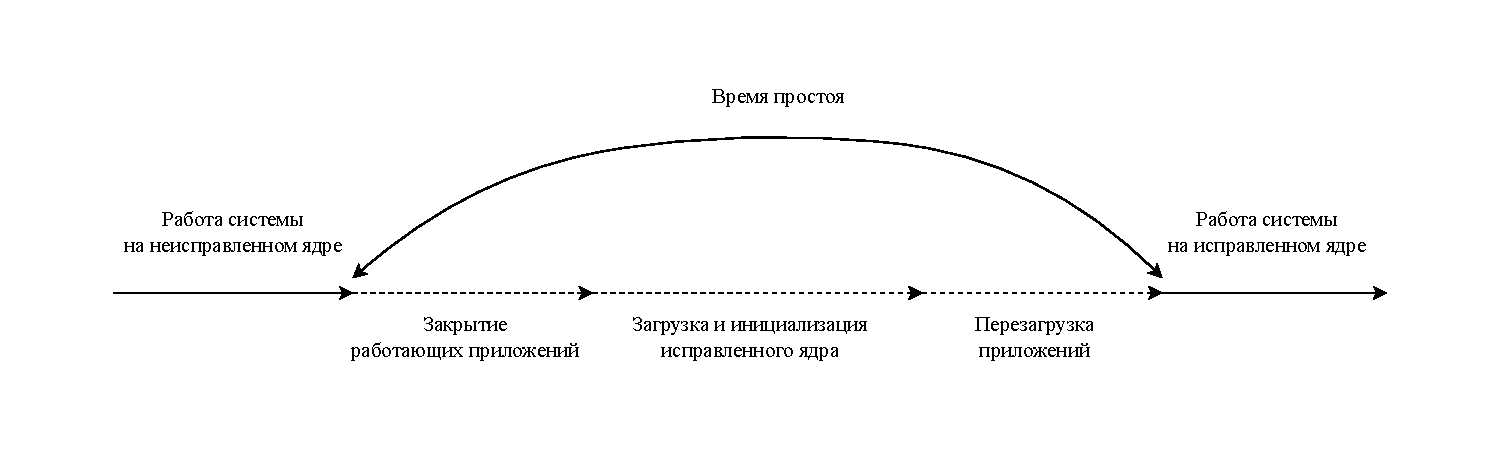
\includegraphics[scale=0.7]{img/downtime.pdf}
	\end{center}
	\captionsetup{justification=centering}
	\caption{Метод, требующий перезагрузки системы}
	\label{img:downtime}
\end{figure}

Для снижения времени простоя появились модификации метода, которые эффективно управляют перезагрузкой ядра. Одна из таких модификаций - бесшовный метод, который сокращает время простоя приложений.

При помощи системного вызова $kexec$ происходит загрузка нового образа ядра. Чтобы применить патч необходимо дождаться момента, когда система примет состояние, в котором выполнены два условия:
\begin{itemize}
	\item все потоки ядра остановлены;
	\item структуры данных ядра согласованны.
\end{itemize}

Выполнение этих двух условий позволяет сделать контрольную точку, которая позволяет сохранить состояние приложений. Код контрольной точки проходит через структуры данных ядра, связанные с приложениями, и преобразует их в высокоуровненый формат, который не зависит от версии ядра. 

После сохранения контрольной точки выполняется инициализация нового ядра. Исправленное ядро считывает контрольную точку и перезапускает приложения, что требует перезагрузки системных вызовов.

Техника бесшовного метода показана на рисунке \ref{img:seemless}.

\begin{figure}[H]
	\begin{center}
		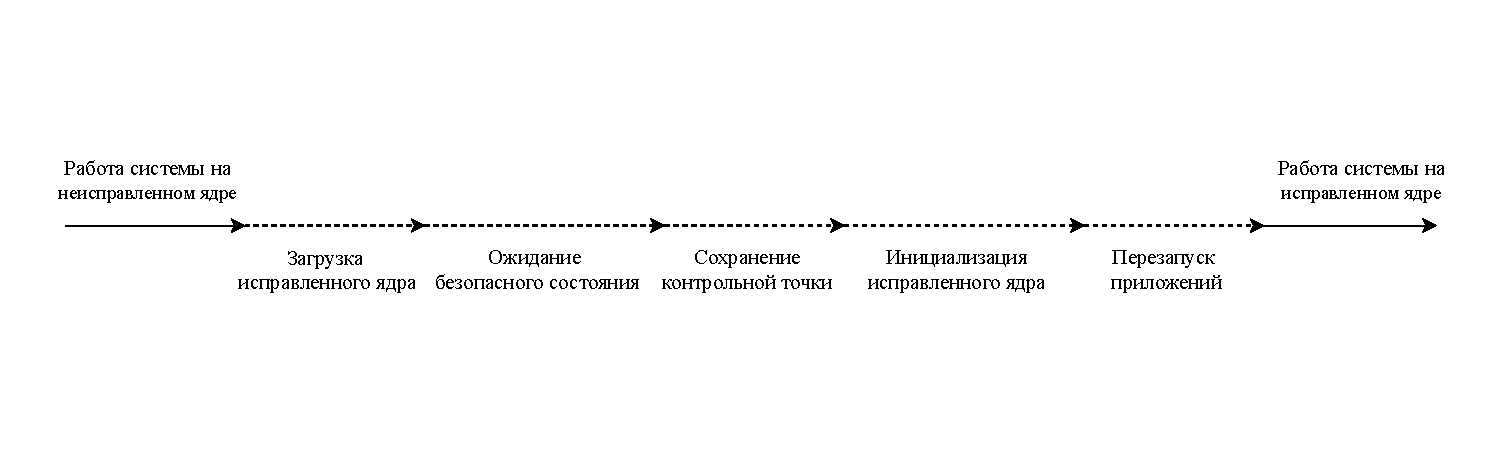
\includegraphics[scale=0.7]{img/seemless.pdf}
	\end{center}
	\captionsetup{justification=centering}
	\caption{Бесшовный метод}
	\label{img:seemless}
\end{figure}

Существует метод, который сокращает время простоя путем одновременного выполнения приложений и перезагрузки системы - метод теневой перезагрузки. Перезагрузка операционной системы выполняется в фоновом режиме на виртуальной машине. Приложения могут продолжать выполняться на исходной машине.

После применения патча на выделенной виртуальной машине, делается его снимок, из которого восстанавливается файловая система.

TODO: рисунок для теневой перезагрузки.

Следующие методы решают проблему простоя исключением перезагрузки системы.

\subsection{Метод переноса}

Идея данного метода \cite{dynamic} заключается в следующем: на другом компьютере запускается измененное ядро, на него переносятся запущенные процессы старого ядра, и оно останавливается. В существующих решениях в качестве другого компьютера используется виртуальная машина, установленная на физической машине, требующей обновления ядра. Необходимо общее хранилище(сервер), которое подключено и к старому, и к новому ядрам. Патч применяется в три этапа.

На первом этапе собирается информация о состоянии операционной системы: подсчитывается число потоков, выполняемых в исправляемом коде, вызывается функция запуска, выполняется инициализация перед передачей управления виртуальной машине.

На втором этапе сервер начинается исправление структур данных и функций. Если измененный модуль не находится в состоянии покоя, обе версии структур данных должны существовать во время процесса исправления. Для обеспечения согласованности структур данных, страницы исходных данных и новых данных защищены. Перехват доступа к ним контролируется виртуальной машиной. То есть, при попытке изменить отслеживаемую страницу управление будет передано виртуальной машине. В этот момент сравнивается содержимое двух версий и вызывается функцию передачи состояния.

На последнем этапе отключается контроль исходных структур данных. Для этого используется метод обхода стека. В случае, если соответствующая исходные структуры используются, адрес возврата исходной функции заменяется адресом функции-заглушки, которые позволяют определить, используется ли еще обновленная функция. Затем выполняется очистка кода старой версии и устанавливается флаг завершения патчинга.

При применении данного метода время простоя невелико. Главным минусом является высокое потребление ресурсов центрального процессора, сети и объема памяти.

TODO: рисунок для переноса.

\subsection{Динамические методы}

Данные методы \cite{dynamic} позволяют применять патчи во время выполнения процессов. Решение состоит из двух этапов.

Для того, чтобы создать измененный код, проводится анализ обновленной и старой	версий. Для этого собирается два варианта ядра: сборка неизмененного кода и сборка измененного кода. В отличие от поиска различий в исходном коде, анализ объектного кода позволяет понять, какие функции были изменены в патче. Большинство функций ядра, которые не были изменены патчем, будут иметь одинаковые объектные коды. Обнаруженные измененные функции помещаются в основной модуль для загрузки в ядро.

Следующий этап необходим для обнаружения встраиваемых функций и неуникальных символов. Для этого проводится сравнение работающего кода ядра и скомпилированного кода. Этот процесс называется предварительным сопоставлением.

Для применения данного метода необходимо определить состояние ядра, когда каждая заменяемая функция будет находиться в состоянии покоя, что является условием безопасного внесения изменений. В этом случае модуль может быть загружен в ядро. Проверка условия безопасного внесения изменений в случае неудачи возобновится через некоторое время. После нескольких неудачных попыток достичь безопасного состояния для применения патча процесс прерывается. Новые инструкции будут вставлены в необновленные функции путем бинарной перезаписи. Бинарная перезапись - это перенаправление вызова функции из исходной в исправленную, для чего используется прыжок к первым пяти или шести байтам функции.

Некоторые решения на основе динамических методов не поддерживают семантические изменения. Кроме того, возникают сложности с изменением типов и структур данных, нестабильных типов данных и функций ядра, которые всегда находятся в стеке вызовов потоков ядра.

Данные методы решают проблему с временем простоя.

TODO: рисунок

\section{Критерии оценки методов}

TODO

\section{Сравнение методов}

TODO

\section{Вывод}

TODO
